\label{sec:hardsoft}
% Our proposed DSLAM system contains two essential improvements on pose estimation and place recognition tasks. As shown in \cref{fig:all_us}, both of these two components are divided into two stages: $1)$ CNN front-end to extract features, deployed on the DPU on PL and $2)$ Algebraic operations to present final results, deployed on the PS ARM cores. To make full use of the Zynq MPSoC, we optimize the data follow for both two components.


\begin{figure}[t]  
    \centering  
    {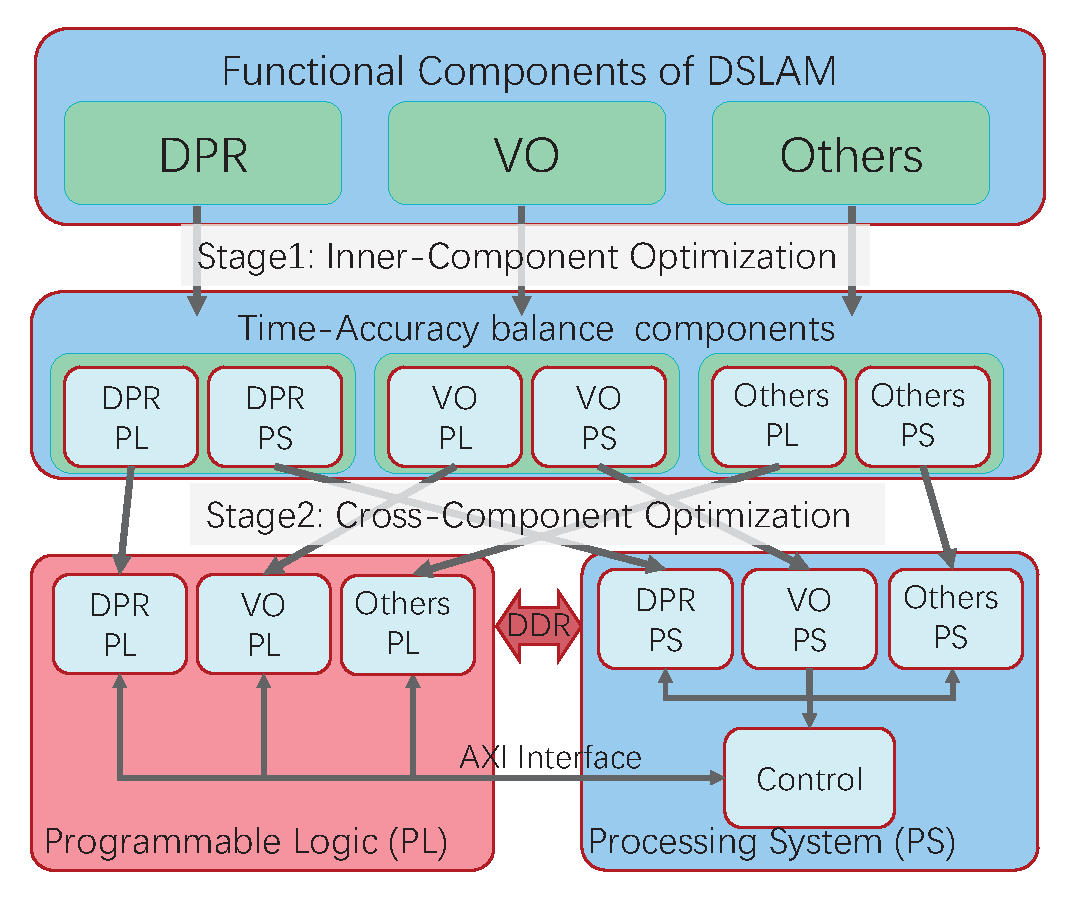
\includegraphics[width=0.9\linewidth]{fig/framework.eps}}
    \caption{The two-stage CNN-based DSLAM framework. Every CNN-based components can be split into two subnets running on PL and PS respectively can can be optimize by the inner-component optimization. The cross-component optimization can effectively schedule the components across PL and PS.}
    \label{fig:framework}
\end{figure}

In this section, we will firstly introduce the two-stage general CNN-based DSLAM framework to leverage the computation resources on embedded FPGA. Then we will take the DSLAM frame shown in \cref{fig:all_us} as an example and introduce the specific implementation of the two stages in this example. 


\begin{figure}[htb]  
    \centering  
    {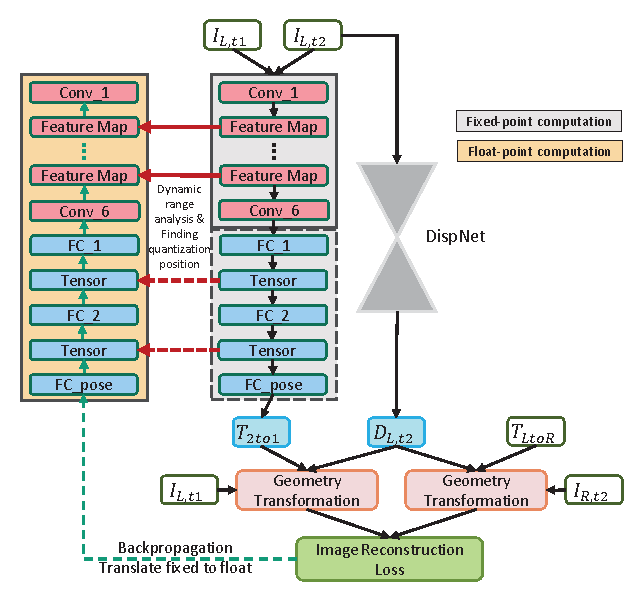
\includegraphics[width=0.9\linewidth]{fig/depth_vo_feat.eps}}
    \caption{Illustration of training framework for visual odometry, where $T_{LtoR}$ is the relative camera pose transformations between left and right views. To speed up the inference, we attepmt different quantization strategies to fixed-finetune the network for VO with fixed-point feed forwarding and floating-point backpropagation.}
    \label{fig:dvo}
\end{figure}


\begin{figure*}[thb]
    \begin{minipage}[t]{0.5\linewidth}  
    \centering
    \subfigure[Scheduling without pipeline. There are only two threads: Camera read and computation.] {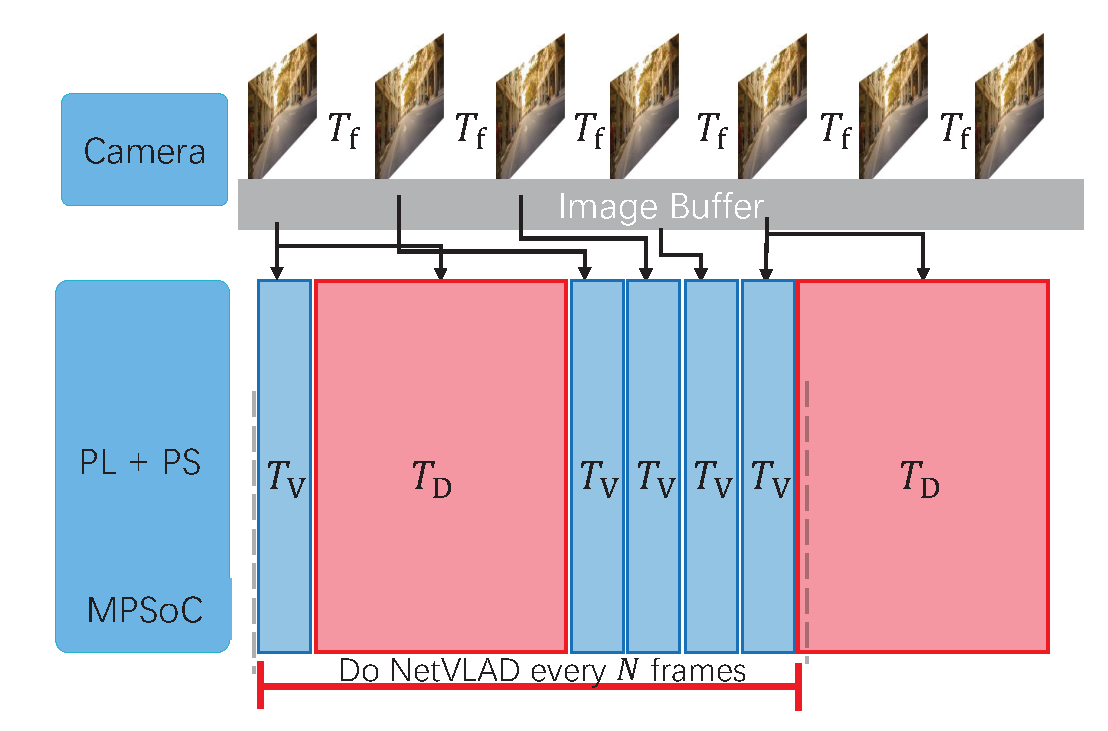
\includegraphics[width=0.85\textwidth]{fig/serial.eps}\label{fig:serial}}
    \end{minipage}
    \begin{minipage}[t]{0.5\linewidth}  
    \centering  
    \subfigure[Scheduling with cross-module pipeline. There are four threads: Camera read, DPU core at PL, PS Operations for VO, and PS Operations for NetVLAD.] {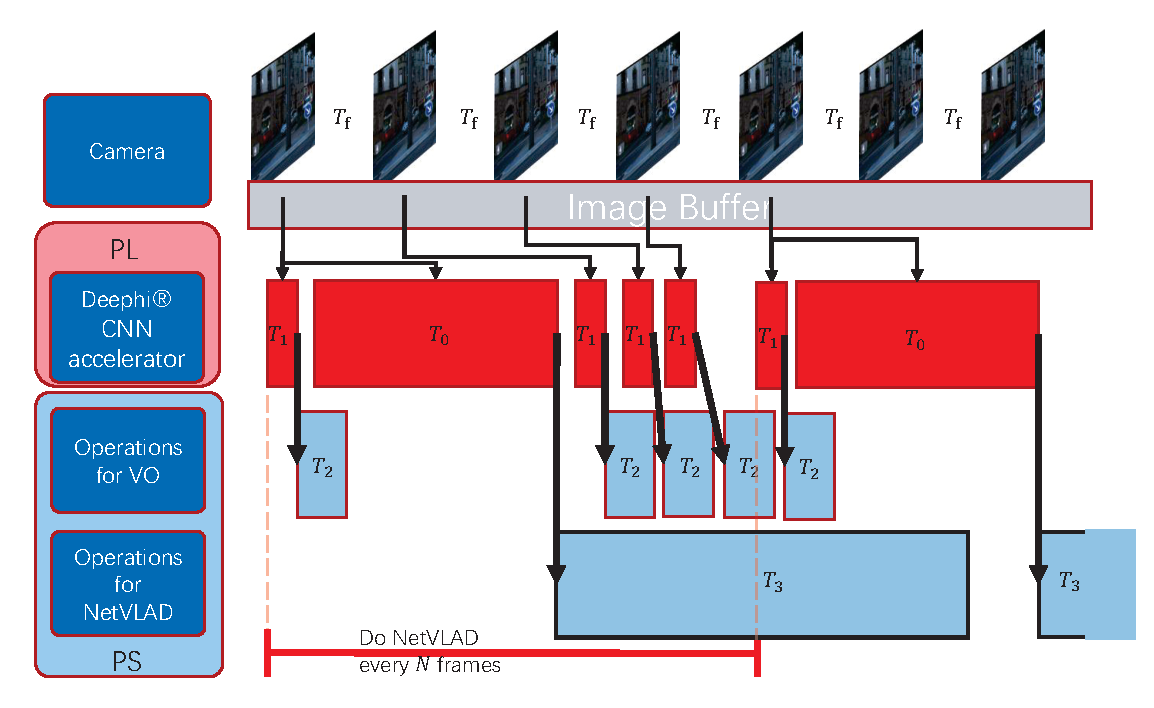
\includegraphics[width=0.85\linewidth]{fig/pipeline.eps}\label{fig:pipline}} 
    \end{minipage}
    \caption{
    The computation pipeline with/without cross-component scheduling.
    }
\label{fig:schedule}
\end{figure*}

\subsection {CNN-based DSLAM framework on FPGA}
As shown in \cref{fig:framework}, our CNN-based FPGA framework contains two major steps: 1) inner-component optimization and 2) cross-component optimization. A DSLAM system has several CNN components such as VO, DPR, and some other components like semantic segmentation which can support the VO and DPR. Each CNN component can and should be divided into two subnets, running on PL and PS side individually. Given the definitive  CNN components, the inner-component optimization stage will find out the balance between the speed and accuracy, and will produce the best split method of each component to PL subnet and PS subnet. After generating the PL and PS subnet for all CNN components, the cross-component optimization stage will schedule the components across the PS and PL in pipeline, so that we can leverage the limited on chip resources and reach the overall optimal system performance. The scheduling configuration and control unit, which will be stored and executed on the PS side, will be generated as the  output of this framework.

In the following subsections, based on the proposed DSLAM method in \cref{fig:all_us}, we will introduce two inner-component method: Pose-Sensitive fixed-point fine-tune method for VO optimization and the NetVLAD  implementation on FPGA for DPR optimization. The cross-component example to scheduling the Depth-VO-Feat and the NetVLAD will be detailed as an example.


\subsection{Pose-Sensitive Fixed-Point Finetune}
% We adopt Depth-VO-Feat \cite{Zhan:2018e92} in DSLAM system to estimate the pose from the input monocular camera. Monocular visual SLAM is a key issue in the field of robotics, while there are two challenging problems: $1)$ it is difficult and expensive to obtain accurate labeled data, $2)$ the methods that use monocular sequences in training always suffer from the scale-ambiguity problem, i.e., the actual scale of translations is missing, and only the direction is learned. Depth-VO-Feat uses image reconstruction loss as a self-supervised signal to train the convolutional neural networks and jointly trains two networks for depth and odometry estimation without external supervision, and solves the two problems. 
% The training framework is illustrated in \cref{fig:dvo}.  


We adopt Depth-VO-Feat \cite{Zhan:2018e92} in the DSLAM system to estimate the pose from the input monocular camera. The training and forwarding framework is illustrated in \cref{fig:dvo}. Depth-VO-Feat uses image reconstruction loss as a self-supervised signal to train the convolutional neural networks and jointly trains two networks for depth (DispNet) and odometry estimation (VONet) without external supervision. In order to run our networks efficiently on the FPGA platform, we use fixed-point arithmetic units on hardware. Previous works use the fixed-point finetune method \cite{Yu:2018:IDC:3299999.3283452} to run CNN in an 8-bit fixed-point arithmetic system without accuracy decline in many applications, such as classification \cite{Qiu:2016151} and object detection \cite{Yu:2018:IDC:3299999.3283452}. Fixed-point fine-tune uses the fixed-point number representation in the feed forward phase and keep floating-point number representation for backpropagation, and both weights and data will be re-quantized after each backpropagation. We find that if the entire VONet is treated as a fixed-point model, the accuracy drops dramatically because VO task requires much higher computational precision than other applications.

Pose-Sensitive fixed-point finetune method can explore the run time of VO at different accuracy. 
We split the VONet into 2 subnets: 1) fixed-point layers for feature extraction. 2) floating-point layers for pose prediction. We propose the \textbf{Pose-Sensitive fixed-point finetune method}, that trains the feature extraction layers with fixed-point finetune method, and trains the pose prediction layers with floating-point.

The Pose-Sensitive fixed-point finetune method will construct some possible network split plans, improve the accuracy under each split plan, and evaluate the run time on the embedded system. With the help of Pose-Sensitive fixed-point finetune, we can balance the accuracy and the execution time. The experiment results of the accuracy and the run time will be exhibited in \cref{sec:experiment}.


%We find out that if we directly consider the whole VO Net as a fixed-point model, the accuracy declines sharply because the VO task requires much more calculation precision than other applications.



% In Depth-VO-Feat \cite{Zhan:2018e92}, we use image reconstruction loss as a self-supervised signal to train the convolutional neural networks and jointly train two networks for depth and odometry estimation without external supervision, which can be used independently in the testing phase. Besides, to fix this scale-ambiguity issue, we use stereo sequences in the training phase and monocular sequences in the testing phase. With the known spatial relationship between the left and right cameras, our neural networks can learn the real world scale. Moreover, we use depth smoothness loss to encourage the predicted depth to be smooth, which demonstrated success in prior works. Then the final loss becomes:

% \begin{equation}
%     L=\lambda_{ir}L_{ir}+\lambda_{ds}L_{ds}
%     \label{equ:loss}
% \end{equation}

% where $L_{ir}$ and $L_{ds}$ are image reconstruction loss and depth smoothness loss respectively, $\lambda_{ir}$ and $\lambda_{ds}$ are the loss weightings for each loss term. 



% Here we adopt the fixed-point finetune method in \cite{Yu:2018:IDC:3299999.3283452}, in that we use the fixed-point number representation in the feed forward phase and keep floating-point number representation for backpropagation, and both weights and data will be re-quantized after each backpropagation. The fixed-point method will lead to a slight accuracy loss of the model, and the performance of the fixed-finetuned Depth-VO-Feat will be shown in detail in \cref{sec:experiment}.

% As the fixed-point method will lead to the accuracy loss of the model, we attempt several different quantization strategies to balance speed and accuracy, which will be shown in detail in \cref{sec:experiment}.

\subsection{DPR on FPGA with NetVLAD}

% \begin{figure}[t]
%     \centering  
%     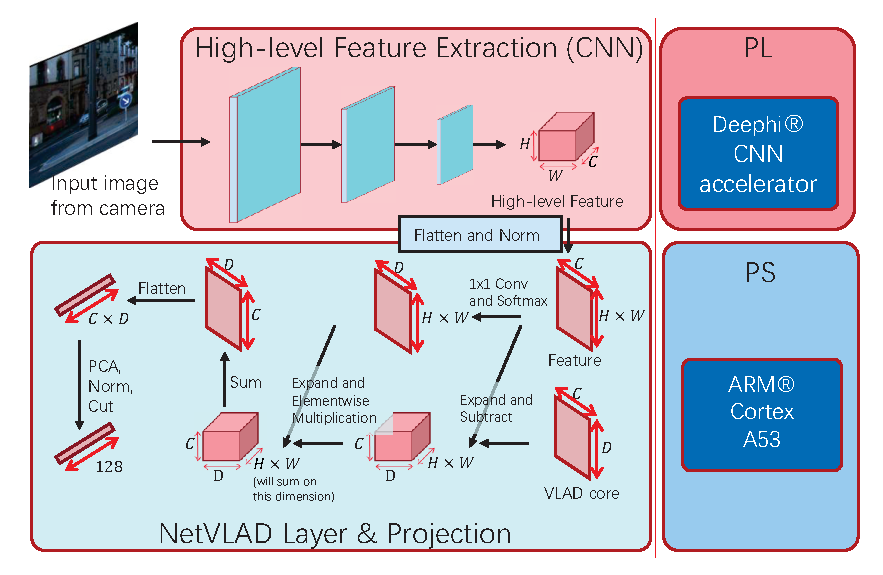
\includegraphics[width=0.95\linewidth]{fig/NetVLAD.eps}
%     \caption{Process of NetVLAD. The CNN encoder is running at the CNN acclerator on PL side, and the VLAD layer as well as the PCA is running at the ARM core at PS side.}
%     \label{fig:NetVLAD}
% \end{figure}

% The place recognition method provide the encoded vector transferred to the central agent for inter-robot place matching. 
The CNN-based DPR methods give the global descriptor of a camera frame in a two-step manner: $1)$ Firstly, a CNN encoder fetches the high-level feature map. $2)$ A vectorization component that aggregates the feature map into a shot global descriptor.
In the original NetVLAD \cite{Arandjelovic:2017997}, the feature extraction encoder is a typical CNN named VGG-16 \cite{Simonyan:20143be}, and the vectorization component consists of VLAD layers.
The PCA method can drastically reduce the output dimension. The previous works \cite{Cieslewski:20187ee,Sarlin:20187ab} show that the 128-D code after PCA is plenty for DSLAM. The VLAD layer and the PCA projection require floating-point number, so we implement the NetVLAD layer and the projection on the PS side of Zynq MPSoC.

% The data flow and operations of the VLAD layer and the projection are complex and require the floating-point number, which cannot be supported with Xilinx DPU. We implement the NetVLAD layer and the projection on the PS side of Zynq MPSoC.

Unlike the fixed-point finetune method used for pose estimation, we simply analyze the dynamic range of the weight and intermediate feature map of each CNN layer, and figure out the optimal decimal point position for each layer respectively to minimize the truncation error of each layer. %\cite{Qiu:2016151}.
% This method is proposed in \cite{Qiu:2016151} and is used in many tasks such as image classification and image detection.

% \begin{figure}[t]
%     \centering  
%     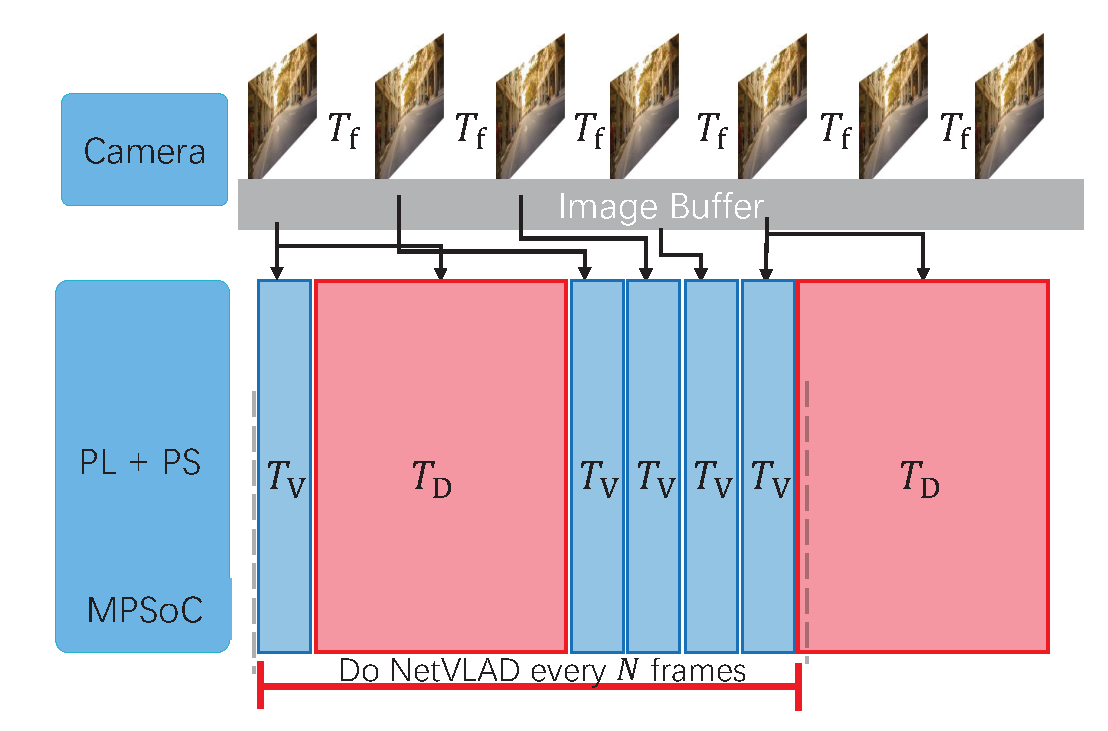
\includegraphics[width=0.95\linewidth]{fig/serial.eps}
%     \caption{Scheduling without pipeline. There are only two threads: Camera read and computation.}
%     \label{fig:serial}
% \end{figure}

% \begin{figure}[t]
%     \centering  
%     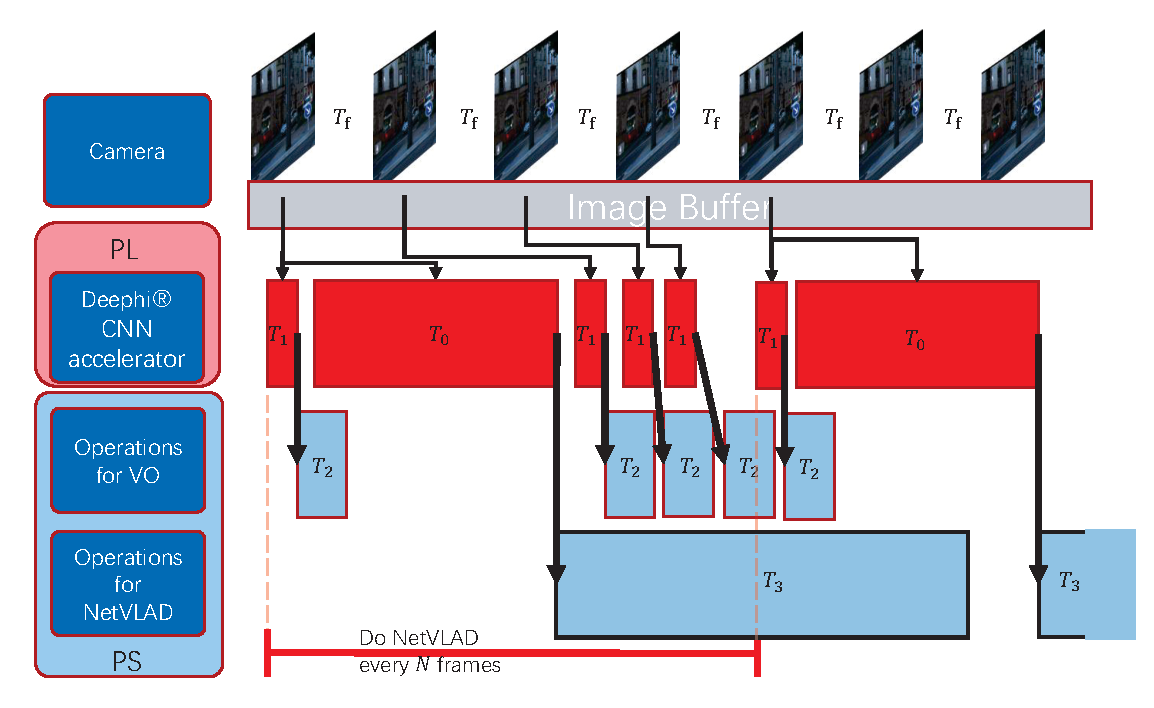
\includegraphics[width=0.95\linewidth]{fig/pipeline.eps}
%     \caption{Scheduling with cross-module pipeline. There are four threads: Camera read, DPU core at PL, PS Operations for VO, and PS Operations for NetVLAD.}
%     \label{fig:pipline}
% \end{figure}


Since the DPU dose not support multi-threading, we can only schedule the whole module of VO and NetVLAD serially. \cref{fig:serial} illustrate the serial schedule strategy. The time interval for reading the camera is $T_{f}$, the VO run time is $T_{V}$ and the NetVLAD run time is $T_{D}$. We do VO every input frame and do NetVLAD every $N$ frames. The $N$ is constrained by \cref{equ:serial}.

\begin{equation}
    N \times T_{f} > T_{D} + N \times T_{V}
    \label{equ:serial}
\end{equation}



\begin{table*}[thb]
  \centering
  \caption{Visual odometry (VO) results on test sequences (09, 10)}
  \footnotesize
  \begin{threeparttable}
\begin{tabular}{|c||cc|cc|cc|c|}
\hline
\multirow{2}[2]{*}{Method} & \multicolumn{2}{c|}{Quant. Strategy} & \multicolumn{2}{c|}{Seq. 09} & \multicolumn{2}{c|}{Seq. 10} & run time  \bigstrut[t]\\
                           & Fixed Part             & Float Part  & $t_{err}^1$        & $r_{err}^1$ & $t_{err}$        & $r_{err}$ & $(ms/frame)$ \bigstrut[b]\\
\hline
ORB-SLAM  & \multicolumn{2}{c|}{-} &15.30 &0.26 &3.68 &0.48 & 230 $^2$ \bigstrut\\
\hline
Depth-VO-Feat\cite{Zhan:2018e92} & \multicolumn{2}{c|}{-} &11.92 &3.60 &12.62 &3.43 & - \bigstrut\\
% Depth-VO-Feat\cite{Zhan:2018e92} & All Float &10.49 &3.34 &11.64 &3.14 &  \bigstrut\\
\hline
\multirow{3}[3]{*}{Ours} & Conv+FC1,2 & FC$\_$pose & 13.27 & 5.27 & 14.75 & 7.78 & 8 \bigstrut\\
% \hline
                         & Conv+FC1 & FC2+FC$\_$pose  & 13.80 & 4.38 & 11.3 & 4.30 & 8 \bigstrut\\
% \hline
                         & Conv & FC1,2+FC$\_$pose &10.27 &4.08 &8.84 &4.01 & 13 \bigstrut\\
\hline
\end{tabular}

\begin{tablenotes}
      \item[1] $t_{err}(\%)$ is the average translational drift error. $r_{err}({}^{\circ}/100m)$ is average rotational drift error.
      \item[2] We run the monocular ORB-SLAM on the PS part of Xilinx ZU9 MPSoC. The run time of reconstructing absolute scale of VO is included. 
      \end{tablenotes}
    \end{threeparttable}
  \label{tab:VO}%
\end{table*}%


\subsection{Cross-Components Scheduling}

The time consumption of NetVLAD and VO is unbalanced. We do pipeline optimization to schedule the two components on Zynq MPSoC efficiently. The pipeline is illustrated in \cref{fig:pipline}. Both NetVLAD and VO time can be divided into two parts: $T_{D} = T_{0} + T_{3},T_{V} = T_{1} + T_{2} $.

The CNN time for NetVLAD and VO is $T_{0}$ and $T_{1}$. The other computation time cost on PS for VO and NetVLAD is $T_{2}$ and $T_{3}$. The frequency of NetVLAD can be expressed as do NetVLAD every $N$ frames $(NetVLAD/\sharp frames)$.


% The constrain of these computation time and $N$ is given as \cref{equ:pipline}.

Considering the thread on PL, the time constraint is given as \cref{equ:pipeline1}. 

\begin{equation}
    N \times T_{f} > T_{0} + N \times T_{1}
    \label{equ:pipeline1}
\end{equation}

The thread for VO on PS constrains the NetVLAD frequency as \cref{equ:pipeline2}.


\begin{figure}[thb]
    \centering  
    \subfigure[Seq. 09] {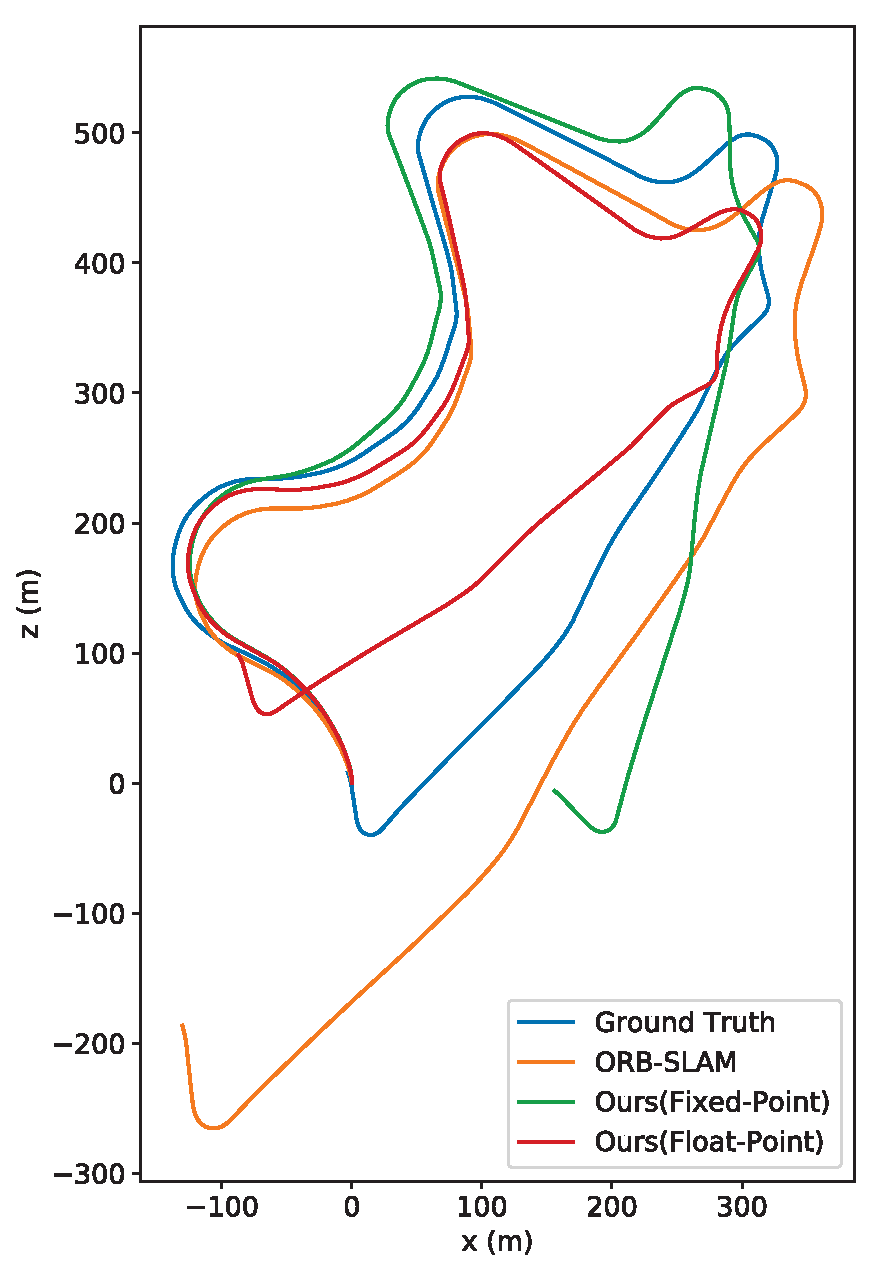
\includegraphics[height=0.7\linewidth]{fig/sequence_09.eps}} 
    \subfigure[Seq. 10] {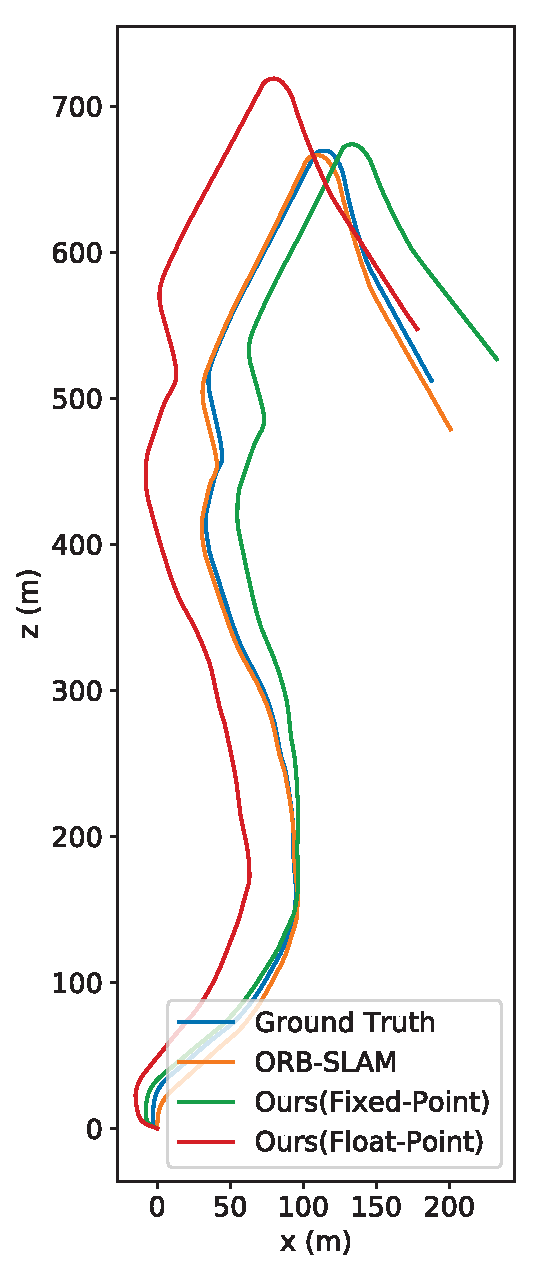
\includegraphics[height=0.7\linewidth]{fig/sequence_10.eps}} 
    \caption{Qualitative evaluation of visual odometry on the KITTI Odometry test sequences (09, 10).}
    \label{fig:VO}
  \end{figure}

\begin{equation}
    N \times T_{f} > T_{0} + T_{1} + (N-1) \times T_{2}
    \label{equ:pipeline2}
\end{equation}

The PS part of current NetVLAD should finish before computing the PS part of next NetVLAD frame. This constraint can be written as \cref{equ:pipeline3}.

% The PS part of NetVLAD should finish before computing the PS part for next NetVLAD frame, and can be writen as \cref{equ:pipline3}.

\begin{equation}
    N \times T_{f} > T_{3}
    \label{equ:pipeline3}
\end{equation}

The execution time of our design will be given in \cref{sec:experiment}.

